\documentclass[@CLASSOPTIONS@]{tumarticle}


\usepackage{cite}
\usepackage{multirow}
\usepackage{hyperref}
\usepackage{graphicx}


\title{Handwritten Mathematical Formula Detection using Deep Learning}

\author[affil={1}, email={niklas.schweiger@tum.de}]{Niklas Schweiger}
\author[affil={1}, email={jannik.obenhoff@tum.de}]{Jannik Obenhoff}

\affil{Department of Electrical and Computer Engineering, Technical
  University of Munich, Arcisstr. 21, 80333 Munich, Germany}

\begin{document}
\twocolumn

\maketitle
\begin{abstract}
  In this analysis project, a data set~\cite{kaggledataset} containing numbers, mathematical
  symbols and letters has been processed in order to train a deep neural network (DNN) that
  serves as a mathematical formula classifier model.
  The final model is applied to real handwritten formulas over a plotly dashboard to demonstrate the model
  performance in the real-world use case.
  In addition, there will be an outlook on future improvements and application scenarios.

\end{abstract}

\section{Introduction}

Handwritten formula detection is a challenging problem in the field of pattern recognition and
image processing.
Despite the recent advancements in machine learning algorithms, different styles, sizes and character
shapes make it difficult to find a perfect detection model.
In this paper, we present a novel approach to handwritten formula detection using convolutional
neural networks (CNNs), image processing, and feature extraction to achieve great results
in real world-scenarios.

\section{Data}
\label{sec:measures}

This section describes the essential preprocessing that has had to be done to the raw
data set~\cite{kaggledataset} before handing it over to the Deep Neural Network,
as well as the scanning process that was made to the real-world data using
various methods like adaptive thresholding.

\subsection{Training Data}
\subsubsection{Understanding and Cleaning the Data}

The training data set contains xxx image samples, all in the 45x45 jpg file format.
The first step was to reduce the data to the necessary characters needed for the
implemented functionalities.
Therefore, characters like the sum formula and more have been removed, limiting the data set
to xxx image samples.

\subsubsection{Preprocessing the Data}

In order to get the best results possible we figured out that the optimal image size would be
28x28 pixels.
After scaling down the samples and first tests, the results were not as desired.
The next preprocessing step was to widen the line thickness of each character.
After some back and forth the optimal line thickness was 6 pixels for the 45x45 jpg samples and
4 pixels for the down sampled 28x28 images.

\begin{figure}[!htb]
   \begin{minipage}{0.24\textwidth}
     \centering
     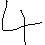
\includegraphics[width=.7\linewidth]{figures/4_clean}
     \caption{Raw Data}\label{Fig:Data1}
   \end{minipage}\hfill
   \begin{minipage}{0.24\textwidth}
     \centering
     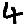
\includegraphics[width=.7\linewidth]{figures/4_sampled}
     \caption{Processed Data}\label{Fig:Data2}
   \end{minipage}
\end{figure}

\subsection{Real Data}
\label{realdata}
Just as with the training data there has had to be done preprocessing before handing
over the real world data to the Machine Learning Model.

\subsubsection{Adaptive Thresholding}

To eliminate distracting background noise an adaptive threshold is applied to the
image.
The first steps are two convolutions with a gaussian kernel with side length 7 (Figure ~\ref{Fig:Data4_1}).
After the convolution the image array gets substituted by 50-minimum value of the original image.
The last step is to threshold the original image with the obtained threshold image.
The result is an image only containing black and white pixels as seen in Figure~\ref{Fig:Data4}.

\begin{figure}[!htb]
   \begin{minipage}{0.48\textwidth}
     \centering
     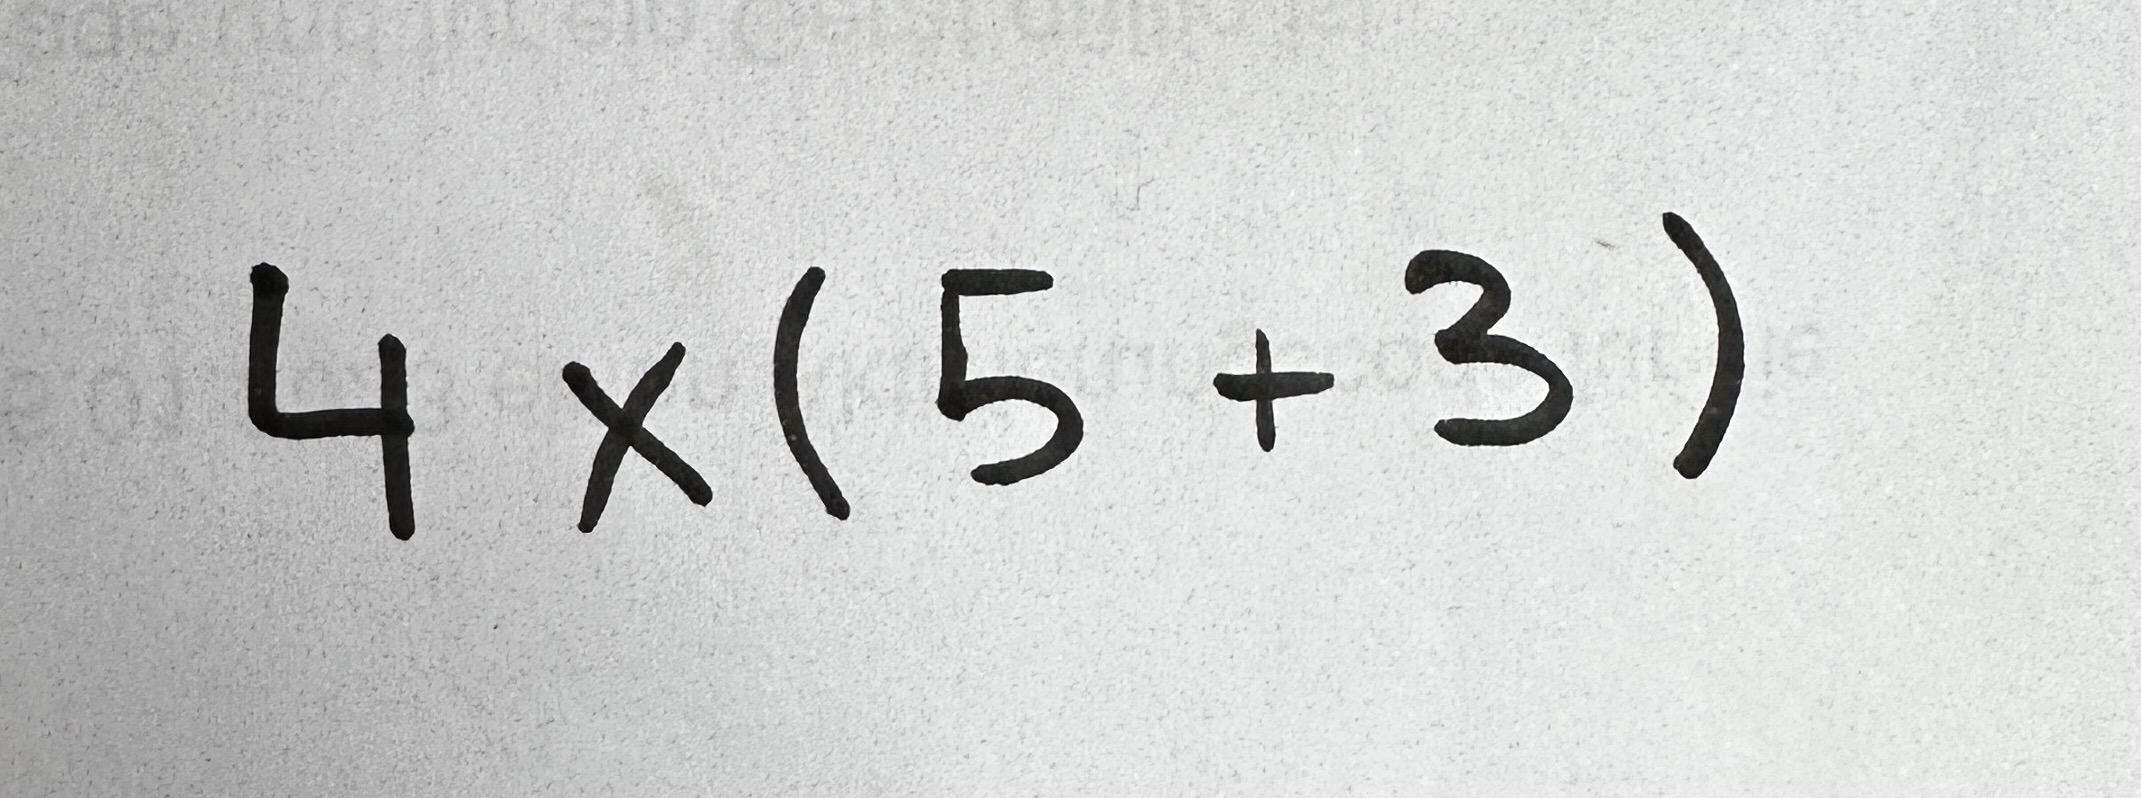
\includegraphics[width=.7\linewidth]{figures/real_data_1}
     \caption{Pre-Thresholding}\label{Fig:Data3}
   \end{minipage}\hfill
   \vspace{0.3cm}
   \begin{minipage}{0.48\textwidth}
     \centering
     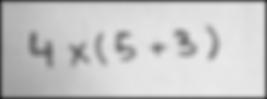
\includegraphics[width=.7\linewidth]{figures/convolve}
     \caption{After-Convolution}\label{Fig:Data4_1}
   \end{minipage}
      \vspace{0.3cm}

   \begin{minipage}{0.48\textwidth}
     \centering
     \fbox{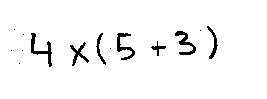
\includegraphics[width=.67\linewidth]{figures/real_data_2}}
     \caption{After-Thresholding}\label{Fig:Data4}
   \end{minipage}
  \hfill
   \begin{minipage}{0.48\textwidth}
     \centering
     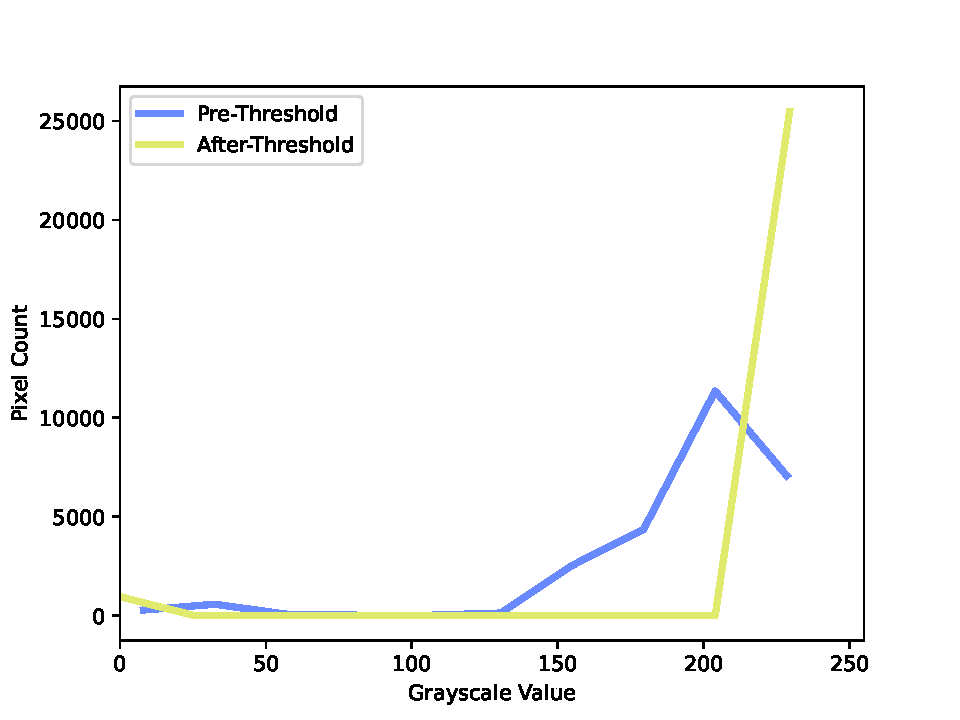
\includegraphics[width=.9\linewidth]{figures/histogram}
     \caption{Pixel Distribution Histogram}\label{Fig:Data5}
   \end{minipage}
\end{figure}

\subsubsection{Scanning and Sampling}

The next step is to scan the image to obtain all individual characters and feed it to the model.
The image array, only containing black and white values, gets scanned by columns to find the starting
and ending column of a character.
To eliminate possible noise, charters only containing one or two columns are being deleted.
After column search, height search is applied to find the character baseline and height.
Every character column gets reduced in size to the maximal height and minimal baseline found in height search.
The second last step is again to eliminate noise, characters with a threshold dimension shape of
min(shape)/max(shape) < 0.1 will get deleted.
The final step is to add an artificial border and to resize every character to a 28x28 image to
perfectly fit the training data see Figure~\ref{Fig:Data6}.

\begin{figure}
    \begin{minipage}{0.48\textwidth}
     \centering
     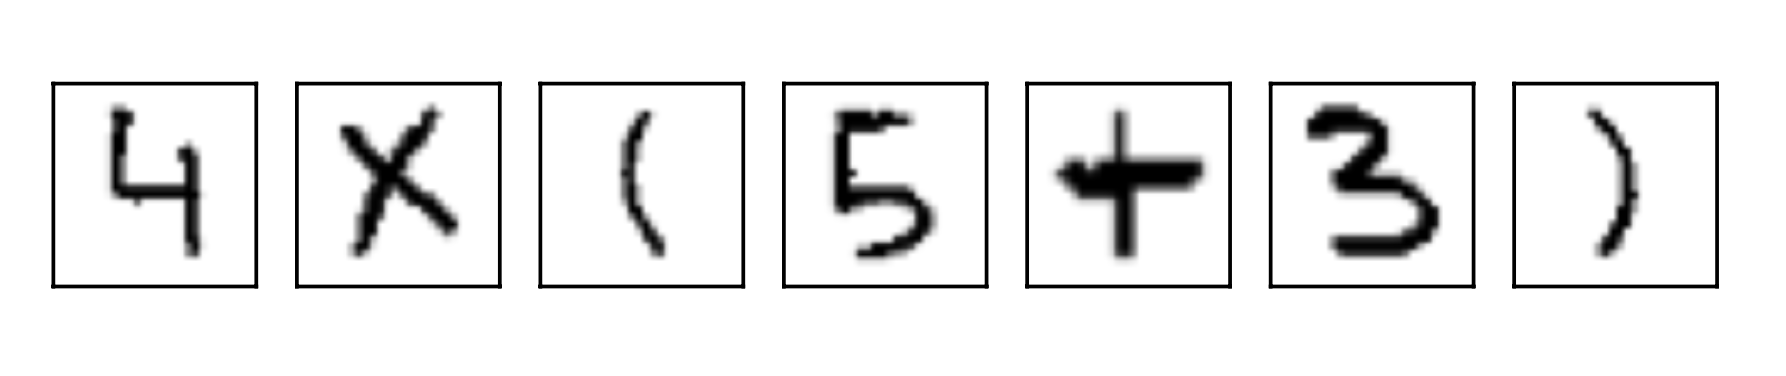
\includegraphics[width=.9\linewidth]{figures/real_data_3}
     \caption{Individual Characters after Scanning}\label{Fig:Data6}
   \end{minipage}
\end{figure}

\section{Model}
\label{sec:implementation}

\subsection{Theoretical background}
Based on the (general and language-agnostic) best practices introduced in
the section above, we implement measures for a C++ software library with
bindings for the Python language in this section.

\subsection{Arcitecture}

The model that has been used for this project is a convolutional deep neural network with a total of six hidden layers.
As only black and white images are passed to the network, the input size is one which connects to ten neurons as
illustrated in figure 4.1. In the first layer each neuron performs a convolution of the input tensor (28 x 28 x 1) with
a kernel size of three and stride and padding of one.After the convolution the ReLU function is used as activation.
In the second layer again a convolution and RELU activation is performed and after that a MaxPool layer with stride and
padding of two which results in a (14 x 14 x 1) tensor at each neuron.The same two layers are then again used for
layers three and four which results in a (7 x 7 x 10) tensor for the whole layer five.The three-dimensional tensors are
then flatted to an (490) array which is necessary because the following SoftMax function requires a one-dimensional
array.Finally, the SoftMax function evaluates a probability for each output class.

\begin{figure}
    \begin{minipage}{0.48\textwidth}
     \centering
     \includegraphics[width=.9\linewidth]{figures/CNN_Architecture}
     \caption{Individual Characters after Scanning}\label{Fig:CNN_A}
   \end{minipage}
\end{figure}

\section{Performance and Results}
\label{sec:customization}

\subsection{Dashboard}

\begin{figure}
    \begin{minipage}{0.48\textwidth}
     \centering
     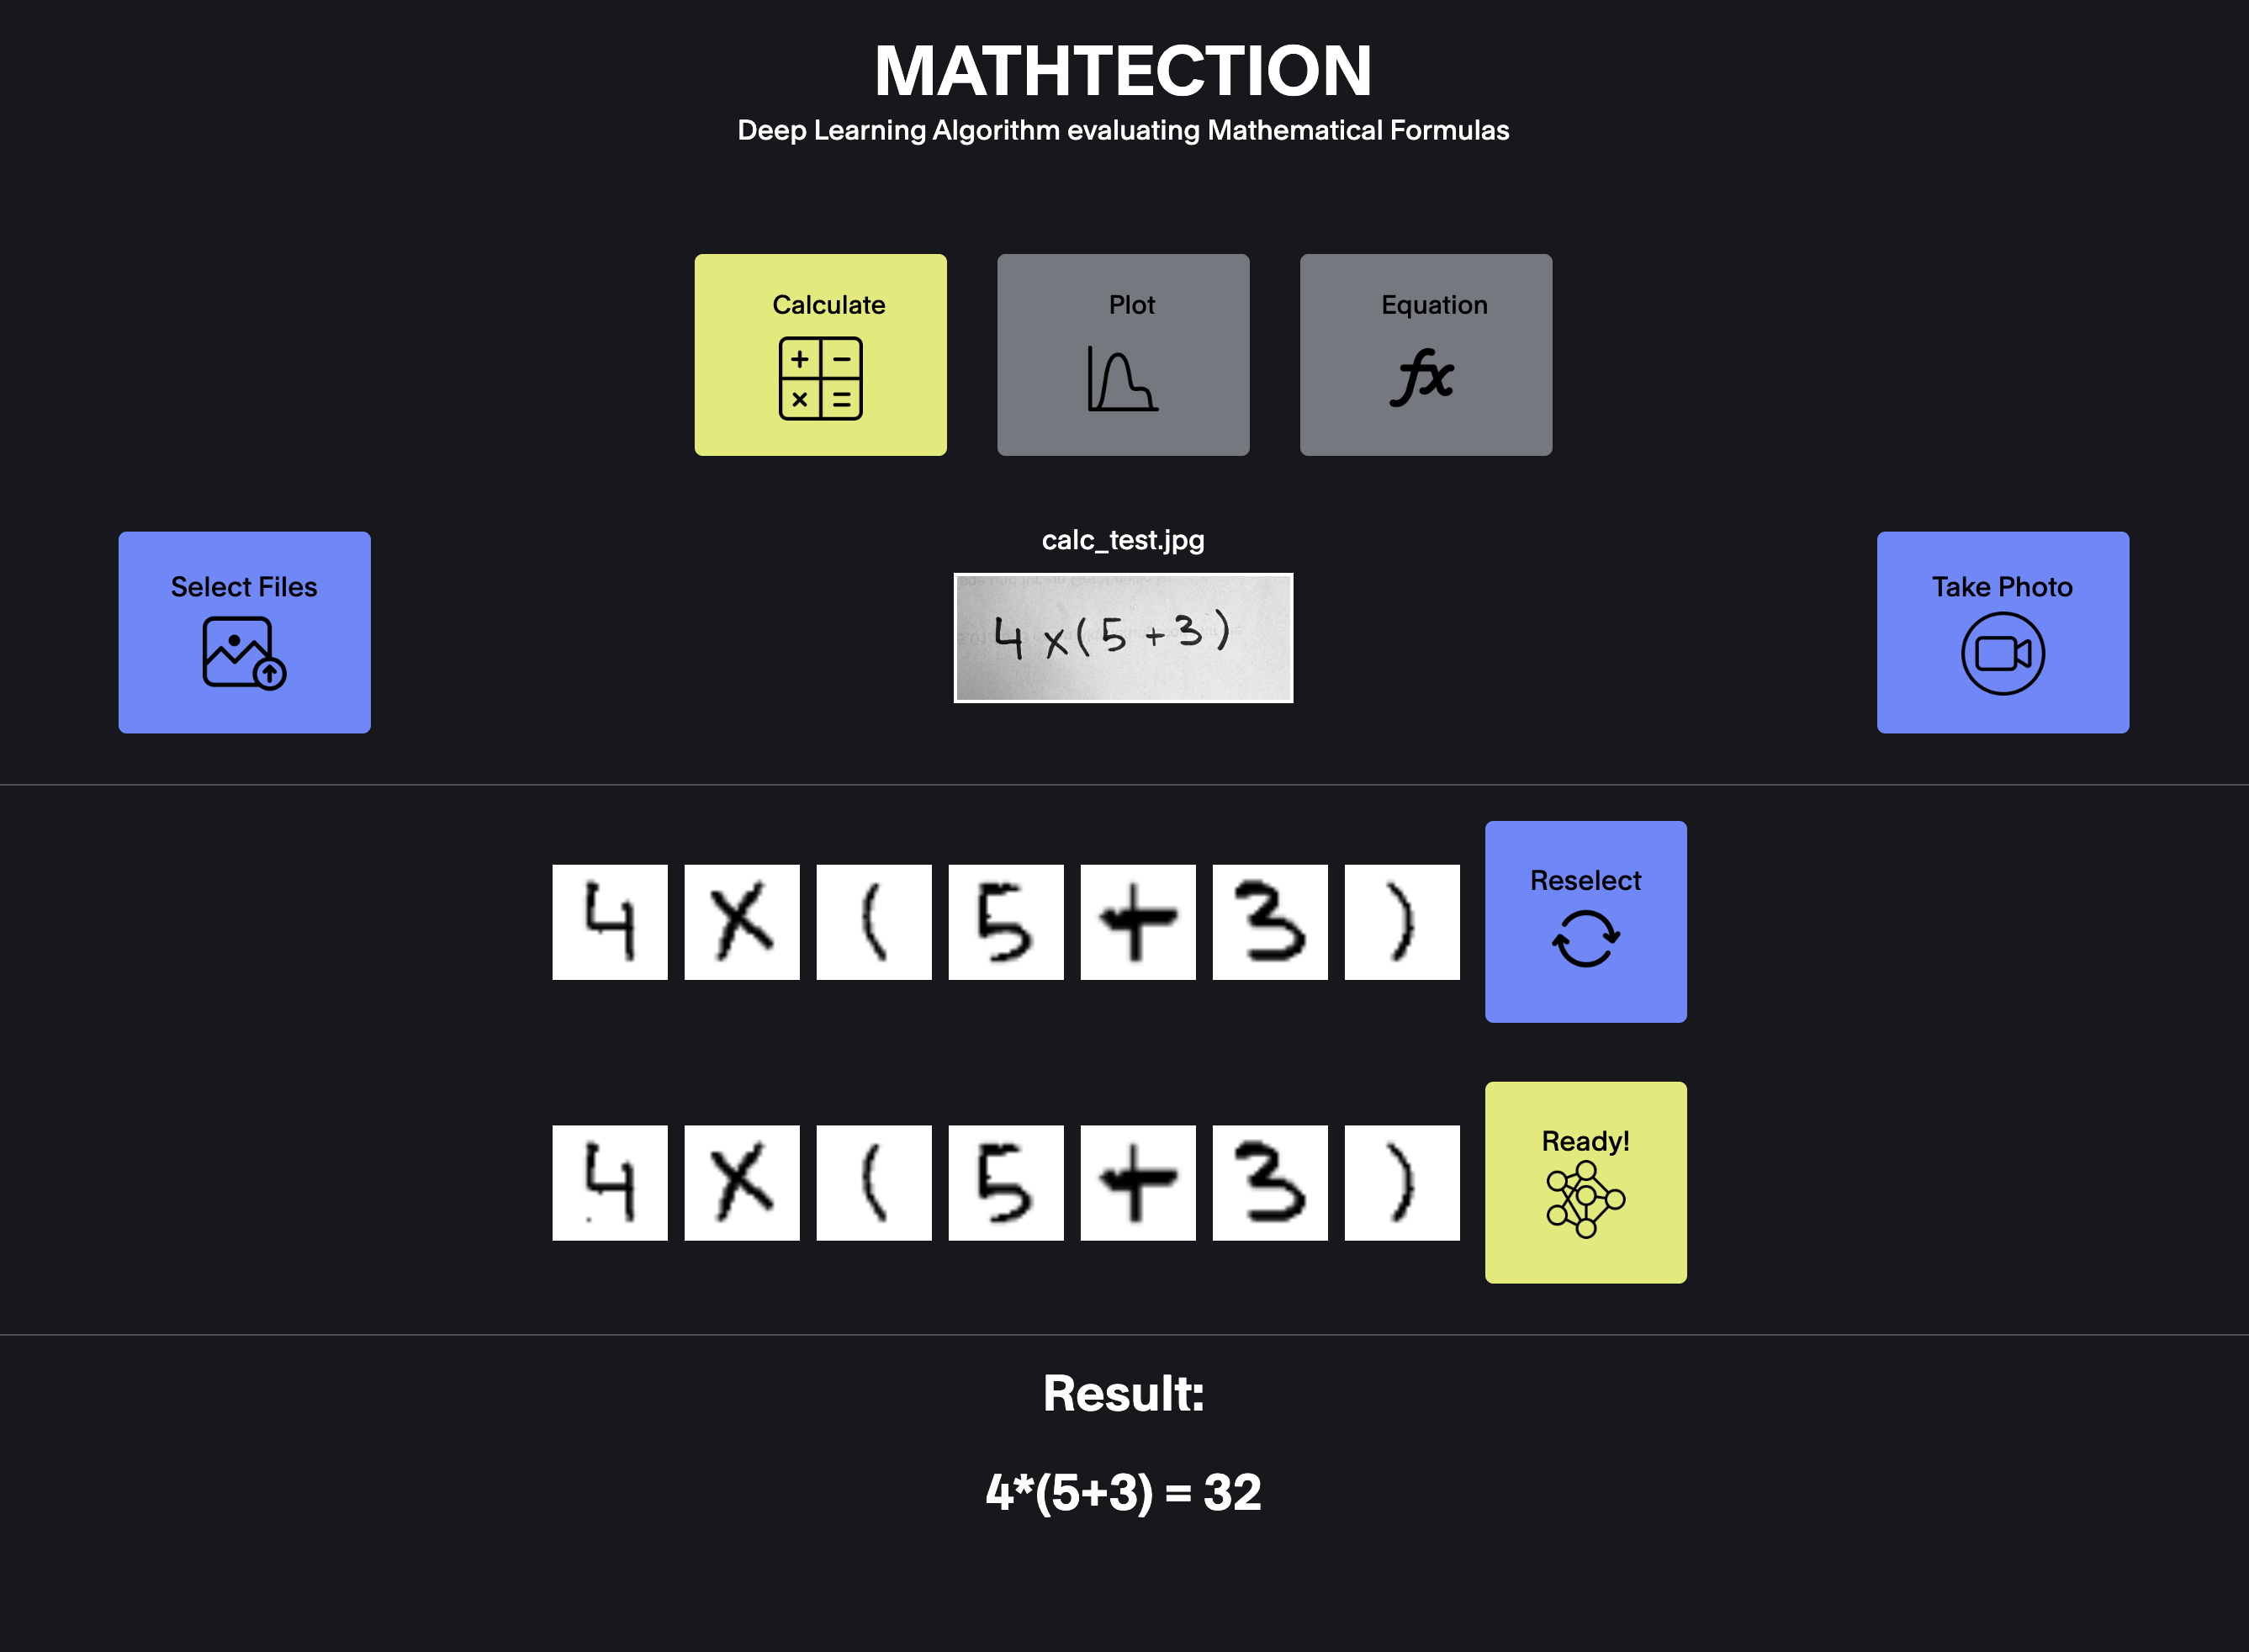
\includegraphics[width=.9\linewidth]{figures/dash}
     \caption{Plotly Dash}\label{Fig:Dash}
   \end{minipage}
\end{figure}

To make easy handling possible a Plotly Dashboard~\cite{plotly} is being used.
The first step for a user is to select one out of three functionalities,
calculation, plotting, equation.
After that it is possible to upload a photo of the handwritten formula or even take a photo
with the webcam.
After the threshold and scanning process\nameref{realdata} the individual characters are displayed
and the user can make a reselection if noise or other undesired parts have been detected.
The final selection gets hand over to the model to classify the characters.
Depending on the selected functionality the result is being displayed.

\section{Outlook and Improvements}

More training data.
Improve model.
Another possible improvement could be to further develop the threshold and scanning process,
to reduce the amount of misidentified characters.
In future the entered real data could be collected in order to extend the training data set for the
Neural Network.

\begin{thebibliography}{10}
  \newcommand{\enquote}[1]{``#1''}

  \bibitem{kaggledataset}
  Xai Nano, \emph{Kaggle Data set: Handwritten math symbols dataset}
  \url{https://www.kaggle.com/datasets/xainano/handwrittenmathsymbols}
  (last accessed: 20.02.2023).

  \bibitem{plotly}
  Plotly \url{https://plotly.com/dash/}
  (last accessed: 07.03.2023).

  \bibitem{hunt1999pragmatic}
  A.~Hunt and H.~Thomas, \emph{The Pragmatic Programmer: From Journeyman to
    Master} (Addison-Wesley, Boston, 1999), 1st ed.

  \bibitem{prlic2012}
  A.~Prli{\'c} and J.~B. Procter, \enquote{Ten simple rules for the open
    development of scientific software,} PLoS Comput. Biol. \textbf{8}, 1--3
  (2012).

\end{thebibliography}

\end{document}
